\documentclass{article}
\usepackage[a4paper, paperwidth=25cm, paperheight=24cm, left=1.5cm, right=1.5cm, top=2cm, bottom=2cm]{geometry}
\usepackage{pgfplots}
\usepackage{tikz,tcolorbox}
\usepackage{listings}
\usepackage{amsmath}
\definecolor{MyBlue}{HTML}{17ADB8}
\definecolor{mypur}{HTML}{A938E1}
\setlength{\parindent}{0pt}

\tcbuselibrary{skins, breakable, theorems}

\lstdefinestyle{cmd}{
 basicstyle=\ttfamily,
 backgroundcolor=\color{lightgray!20},
 frame=single
}

\lstdefinestyle{javaStyle}{
    language=Java,
    basicstyle=\ttfamily\footnotesize,   % Font style and size
    numbers=left,                       % Line numbers on the left
    numberstyle=\tiny\color{gray},       % Style for line numbers
    stepnumber=1,                        % Line number step
    numbersep=5pt,                       % Distance of numbers from the code
    backgroundcolor=\color{white},       % Background color of the listing
    showspaces=false,                    % Don't show spaces
    showstringspaces=false,              % Don't show spaces in strings
    showtabs=false,                      % Don't show tab characters
    frame=single,                        % Add a frame around the code
    rulecolor=\color{black},             % Color of the frame
    tabsize=2,                           % Tab size
    captionpos=b,                        % Position of the caption (bottom)
    breaklines=true,                     % Automatically break long lines
    breakatwhitespace=true,              % Break at white space
    escapeinside={\%*}{*)},              % Allows comments in LaTeX inside the listing
    keywordstyle=\color{blue},           % Keyword color
    commentstyle=\color{green},          % Comment color
    stringstyle=\color{red},             % String color
}

\newtcolorbox{prettyBox}[2]{
  enhanced,
  colback=white!90!#2,   % Background color based on the second parameter (color)
  colframe=#2!60!black,  % Frame color based on the second parameter (color)
  coltitle=white,        % Title color (white)
  fonttitle=\bfseries\Large,
  title=#1,              % Title from the first parameter
  boxrule=1mm,
  arc=0.5mm,
  drop shadow=#2!35!gray, % Drop shadow color based on the second parameter (color)
}



\begin{document}
\begin{center}
    \Huge{\textbf{\underline{Chapter 1: Introduction}}}
\end{center}

\setcounter{section}{0}

\vspace{0.35cm}

\section{Steps Of An Attack}

\vspace{0.25cm}
\begin{center}
    \includegraphics[width=0.9\textwidth]{Chapters/Diagram/Introduction/attack.drawio.pdf}
\end{center}

\vspace{0.35cm}
\section{Reasons for Poor Security}
\begin{prettyBox}{Reasons}{myblue}
\begin{itemize}
    \item \textbf{Insufficient Budget}: Approximately \(\frac{1}{4}\) of issues arise due to inadequate funding for cybersecurity initiatives and personnel.
    \item \textbf{Unqualified Personnel}: A lack of skilled and properly trained cybersecurity professionals.
    \item \textbf{Poor Administration}: Inefficient management and lack of synchronization in security policies and practices.
\end{itemize}
\end{prettyBox}

\vspace{0.35cm}

\section{Impacts of a Cyberattack}
\begin{prettyBox}{Impacts}{myblue}
\begin{itemize}
    \item \textbf{Data Breach}: Unauthorized access to sensitive client or organizational data. This may include\\ encrypting data for ransom (ransomware), sharing confidential information, or selling it on the dark web.  
    \item \textbf{Denial of Service (DoS)}: Disrupting or halting the services of an organization, making them inaccessible to users.   
    \item \textbf{Financial Loss}: Hacking into bank accounts, demanding ransom (ransomware attacks), or causing service interruptions that result in revenue loss.  
    \item \textbf{Damage to Reputation}: Eroding client trust or tarnishing someone's reputation by exposing compromised or sensitive data.  
    \item \textbf{Loss of Clients}: Organizations may lose clients due to the exposure of sensitive information, compromised systems, server outages, and interruptions in services.  
\end{itemize}
\end{prettyBox}

\newpage

\section{Information System}
\begin{prettyBox}{Definition}{myblue}
A set of active applications, services, and other components that allow for the management of informations.
Vulnerabilities can affect all components of the information system (IS).  
\end{prettyBox}

\section{Responses to Cyberattacks}
\begin{prettyBox}{Responses}{myblue}
\begin{itemize}
    \item \textbf{Reduce the Impact}: Taking measures to minimize the damage caused by the cyberattack, such as isolating affected systems, restoring backups, or limiting access.  
    \item \textbf{Accept the Risk}: The least effective response, where no action is taken to counter the attack. This could include surrendering to attackers’ demands, such as paying a ransom.  
    \item \textbf{Refuse or Resolve the Risk}: Actively countering the attack by refusing to comply with attackers and taking corrective actions to fix vulnerabilities or breaches.  
    \item \textbf{Transfer the Responsibility}: Shifting the burden of dealing with the cyberattack to a third party, such as an insurance provider or a managed cybersecurity service.  
\end{itemize}
\end{prettyBox}

\vspace{0.5cm}

\section{Steps For Protection (Deming's Wheel)}
\begin{prettyBox}{PDCA}{myblue}
    The PDCA (Plan-Do-Check-Act) cycle is a continuous improvement process widely used in
cybersecurity to ensure effective protection and adapt to evolving threats. Below are the four key steps:

    \begin{itemize}
        \item \textbf{\textcolor{green}{P}lan}: Identify goals, assess risks, and develop strategies to strengthen cybersecurity.
        \item \textbf{\textcolor{green}{D}o}: Implement the cybersecurity measures, like deploying firewalls and training staff.
        \item \textbf{\textcolor{green}{C}heck}: Monitor and evaluate the effectiveness of security measures through audits and testing.
        \item \textbf{\textcolor{green}{A}ct}: Address weaknesses and refine security measures to adapt to new threats.
    \end{itemize}
\end{prettyBox}

\begin{center}
    \includegraphics[width=0.5\textwidth]{Chapters/Diagram/Introduction/pdca.drawio.pdf}
\end{center}



\section{Software Crisis}
\subsection{Birth Of Software Enginner}
\subsection{Qualities Of A Software}

\section{Life Cycle Of Software}
\subsection{Whats's Life Cycle Of Software?}
As the name suggest it's the life cycle of a software from start to finish , life cycle also known as model is a methodology
that serves to help developers in building their product , each life cycle has steps and a chronology to follow
\subsection{WaterFall Life Cycle}
\subsubsection{First Version}
\vspace{0.5cm}
\begin{tikzpicture}
    \draw (-1,0) rectangle (3.5,1.5);
    \node at (1.25,0.75) {Definition \& Needs Analysis};

   \draw[->] (3.5,0.75) -- (5,0.75) -- (5,0);

    \draw (4,-1.5) rectangle (6,0);
    \node at (5,-0.75) {Conception};

    \draw[->] (6,-0.75) -- (7.5,-0.75) -- (7.5,-1.5);

    \draw (6.5,-3) rectangle (8.5,-1.5);
    \node at (7.5,-2.25) {Coding};

    \draw[->] (8.5,-2.25) -- (10,-2.25) -- (10,-3);

    \draw (9,-4.5) rectangle (11,-3);
    \node at (10,-3.75) {Testing};

    \draw[->] (11,-3.75) -- (13.75,-3.75) -- (13.75,-4.5);

    \draw (11.5,-6) rectangle (16,-4.5);
    \node at (13.75,-5.25) {Deployment \& Maintenance};
\end{tikzpicture}
\subsubsection{Improved Version}
\vspace{0.5cm}
\begin{tikzpicture}
    \draw (-1,0) rectangle (3.5,1.5);
    \node at (1.25,0.75) {Definition \& Needs Analysis};

   \draw[->] (3.5,0.75) -- (5,0.75) -- (5,0);

    \draw (4,-1.5) rectangle (6,0);
    \node at (5,-0.5) {Achitectural};
    \node at (5,-1){Design};
    \draw (4,-3) rectangle (6,-1.5);
    \node at (5,-2) {Detailed};
    \node at (5,-2.5) {Design};

    \draw[->] (6,-1.5) -- (7.5,-1.5) -- (7.5,-2);

    \draw (6.5,-3.5) rectangle (8.5,-2);
    \node at (7.5,-2.75) {Coding};

    \draw[->] (8.5,-2.25) -- (10,-2.25) -- (10,-3);

    \draw (9,-4.5) rectangle (11,-3);
    \node at (10,-3.75) {Unit Test};
    \draw (9,-6) rectangle (11,-4.5);
    \node at (10,-5) {Integration};
    \node at (10,-5.5) {Test};

    \draw[->] (11,-4.5) -- (13.75,-4.5) -- (13.75,-5);

    \draw (11.5,-6.5) rectangle (16,-5);
    \node at (13.75,-5.75) {Deployment \& Maintenance};
\end{tikzpicture}
\subsection{V Life Cycle}
\subsection{Prototyping Life Cycle}
\subsection{Incremental Life Cycle}
\subsection{Spiral Life Cycle}
\subsection{Hybrid Life Cycle}

\section{Needs Analysis}
A thorough needs analysis is critical in software development. Any ambiguity, contradiction, or missing information found in the
requirements document can lead to significant setbacks, potentially requiring a restart of the project. In this section, we will
take a detailed look at how the requirements document is structured.

\begin{prettyBox}{Note}{red} 
\textbf{Difference Between Goals \& Needs ?}\\

It is crucial to understand that the requirements document holds the client's needs and not their goals . A goal is subjective and
open to interpretation, while a need is objective—measurable or verifiable.\\

\textbf{\underline{Example :}}\\

The client might request a "pleasant user interface" , This can be interpreted in many ways:
\begin{itemize}
    \item a visually appealing UI with lots of colors and animations   
    \item an easy-to-use interface
    \item a minimalistic design
\end{itemize} 

and so on. To turn this into a clear need, we must clarify what the client means. For instance, they might want the UI to be 
organized with all features accessible through a dropdown menu.

\end{prettyBox}

\subsection{Requirments Document Structure}
\begin{itemize}
   \item \textbf{Introduction : }This section provides an overview of the document by outlining its key components :
      \begin{itemize} 
          \item Purpose: The reason for creating this document, which is primarily to align the development team and facilitate
           communication with the client.
           \vspace{0.15cm}
          \item Scope: A high-level summary of the software’s main functionality, without going into too much detail. 
           \vspace{0.15cm}
          \item Context: The reason for creating the software, which could be to sell it to a client or company, to develop an
          open-source project, or other similar motivations.\\
      \end{itemize}    
    \item \textbf{Hardware : }This section states whether the software requires any special hardware components like : GPU,
sensors, or a camera ...etc . It also outlines the minimum hardware requirements needed to run the software, as well as the optimal hardware configuration for the best and smoothest experience.
    \item \textbf{Conceptual Model : }This section describes the overall software architecture through a high-level graphical
        representation, highlighting key components and their relationships.\hspace{0.1cm}It provides an overview of how the system is structured and
operates, making it easier for stakeholders to understand.

\textbf{\underline{Example :}}

A desktop system composed of an email service, a spreadsheet, a document processing service, and an information retrieval service.
\end{itemize}
\begin{center}
\begin{tikzpicture}
    \draw (0,0) rectangle (2,1);
    \node at (1,0.5){User};
    \draw[->] (1,1) -- (1,2) -- (10.5 ,2) -- (10.5,-2);
    \draw[->] (2,0.5) -- (6.25,0.5) -- (6.25,0);
    \draw[->] (0,0.5) -- (-1.5,0.5) -- (-1.5,-8) -- (1.75,-8) -- (1.75,-7);
    \draw[->] (1.625,0) -- (1.625,-1);

    \draw (0.5,-3) rectangle (2.75,-1);
    \node at (1.625,-1.75) {Email};
    \node at (1.625 ,-2.25){Management};
    \draw[->] (1.625,-3) -- (1.625,-4);
    \draw[->] (0.5,-2) -- (-0.5,-2) -- (-0.5,-6.5) -- (0.75,-6.5);
    \draw[->] (2.75,-2) -- (4.125,-2) -- (4.125,-1) -- (5.25,-1);

    \draw (0.75,-5) rectangle (2.75,-4);
    \node at (1.75,-4.5) {Network};

    \draw (0.75,-7) rectangle (2.75,-6);
    \node at (1.75,-6.5) {Spreadsheet};
    \draw[->] (2.75,-6.5) -- (5.25,-6.5);
      
    \draw (5.25,-7) rectangle (7.25,-6);
    \node at (6.25,-6.5) {DB};

    \draw(5.25,-2) rectangle (7.25,0);
    \node at (6.25,-0.75) {Document};
    \node at (6.25,-1.25) {Processing};
    \draw[->] (6.25,-2) -- (6.25,-6); 
  
    \draw (9.5,-4) rectangle (11.5,-2);
    \node at (10.5,-2.75) {Information};
    \node at (10.5,-3.25) {Retrieval};
    \draw[->] (10.5 , -4) -- (10.5,-6.5) -- (7.25,-6.5); 

 \end{tikzpicture}
\end{center}

\vspace{0.75cm}
The next step consist into creating a new conceptual model for each complexe fonction
\vspace{0.25cm}
\begin{center}
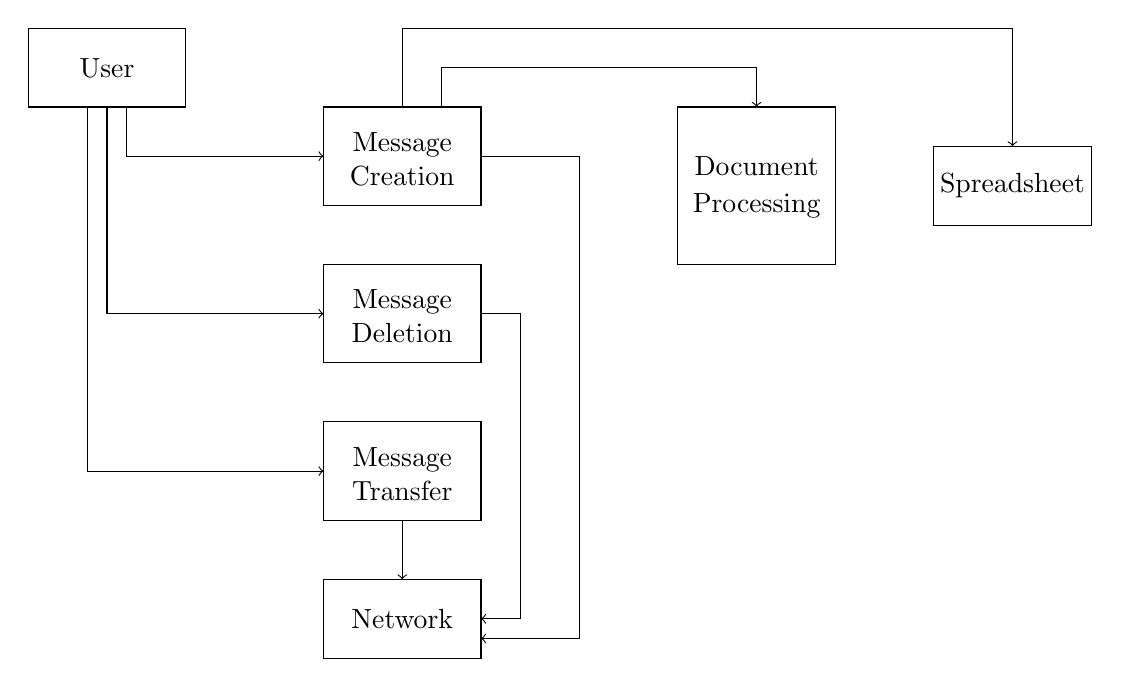
\begin{tikzpicture}
    \draw (-3,0) rectangle (-1,1);
    \node at (-2,0.5){User};
    \draw[->] (-2,0) -- (-2,-2.625) -- (0.75,-2.625);
    \draw[->] (-1.75,0) -- (-1.75,-0.625) -- (0.75,-0.625);
    \draw[->] (-2.25,0) -- (-2.25,-4.625) -- (0.75,-4.625);
    
    \draw (0.75,-1.25) rectangle (2.75,0);
    \node at (1.75,-0.475){Message};
    \node at (1.75,-0.875){Creation};
    \draw[->] (2.75,-0.625) -- (4,-0.625) -- (4,-6.75) -- (2.75,-6.75);
    \draw[->] (2.25,0) -- (2.25,0.5) -- (6.25,0.5) -- (6.25,0);
    \draw[->] (1.75,0) -- (1.75,1) -- (9.5,1) -- (9.5,-0.5);

    \draw (0.75,-3.25) rectangle (2.75,-2);
    \node at (1.75,-2.475){Message};
    \node at (1.75,-2.875){Deletion};
    \draw[->] (2.75,-2.625) -- (3.25 ,-2.625) -- (3.25,-6.5) -- (2.75,-6.5);

    \draw (0.75,-5.25) rectangle (2.75,-4);
    \node at (1.75,-4.475){Message};
    \node at (1.75,-4.875){Transfer};
    \draw[->] (1.75,-5.25) -- (1.75,-6);

    \draw (0.75,-7) rectangle (2.75,-6);
    \node at (1.75,-6.5) {Network};

    \draw (8.5,-1.5) rectangle (10.5,-0.5);
    \node at (9.5,-1) {Spreadsheet};
    
    \draw(5.25,-2) rectangle (7.25,0);
    \node at (6.25,-0.75) {Document};
    \node at (6.25,-1.25) {Processing};

\end{tikzpicture}

\end{center}
\begin{itemize}
\item \textbf{Functional Requirements:} These define what the system should do, focusing on the specific features and functions the
software must deliver to meet user or business needs. They describe the expected behavior of the system in various situations.
Functional requirements are concrete and measurable. They can be expressed using natural, semi-formal, or formal language,
or a mix of these. 

\begin{itemize} 
\item \textbf{Natural Language:} Easy to implement and understand, but lacks structure and precision, which can lead to ambiguity.
It makes automating analysis of the document harder, relying heavily on the writer’s linguistic experience. 
\item \textbf{Structured (Semi-Formal) Language:} Limited use of natural language, more structured and precise than natural language
, often accompanied by graphical notations. 
\item \textbf{Formal Language:} Hard to master and time-consuming to implement. It is difficult for clients to understand but is based
on mathematical theory, making it the most precise language and easier to automate verification. 
\end{itemize}

\item \textbf{Non-Functional Requirements:} Define the restrictions and constraints related to both hardware and software within
the context of the ongoing project. Non-functional requirements are particularly influenced by changes in technologies 
(both hardware and software) and are crucial for complex software systems. As the project develops, changes in hardware may occur.
These changes can be anticipated by projecting the expected performance levels that will be required by the end of the project.
\item \textbf{Maintenance Information:} Anticipates possible actions after the software's initial release, such as adding
new features, improving performance, or addressing potential issues.
   \item \textbf{Glossary:} Provides definitions of the terms and concepts used in the document to help readers. This ensures
that the terminology is clear, as the requirements document is shared and read by the design team, developers, and stakeholders, 
without assuming prior knowledge of these terms.
  \item \textbf{Index:} Helps the reader find specific topics and sections of the document more efficiently by providing a
detailed list of references to relevant sections, parts, and page numbers.
\end{itemize}


\begin{prettyBox}{Note}{red}
 Functional and non-functional requirements are inherently connected, and their interplay can sometimes lead to conflicts. 
 By understanding the potential for these conflicts and establishing a process for managing them, development teams can better
 balance user needs and system performance, ultimately leading to a more successful product.
\end{prettyBox}

\subsection{Requirements Validation}
The requirements need to be coherent, realizable, and complete. Anticipation of hardware needs to be considered. 
It is crucial for the requirements document to be validated in order to initiate the next steps of the software life cycle.

\begin{itemize}
    \item review Technique is an efficient way to monitor and update the requirements .
    \item There are various analysis tools available that can facilitate the validation process of the requirements document,
helping to ensure accuracy and completeness.
\end{itemize}


def UML :

Type Of uml diagram


UML semi formel 

categorizes into two :
structure : diagram de class solution OOP 
Comportement :

use case diagram :

actor : user , hardware , other software 

note : 
one person can play many rols 

cas d'utilisation = features = elipse
bonhome = actor
mix of natural language , and graphical symbols
associate actor with use case with line

use case : is a graphical representation of a behaviour diagram
that is composed of actors that can be huaman (intern,externe) , or 
non human hardware that interact with the software , or other softwares
, each actors has one or many rols we create links called association between actors and use case 
(softwares features)

type of relation 
association : actor ---> use case

possible relation between use case and use case
relation between softwares features

generalisation <=> looks like extend relation
remarque : relation can be applied on actors too

                     extends
extention : source ----------> detination
if condition == true execute source use case 
case extention

                     include
inclusion : source ----------> detination

if actor want to do source use case he has to do destination use case first
only applied between user case 

note :
difference between inclusion and extension

\section{Conception}

\subsection{Introduction}
\begin{prettyBox}{Conception Introduction}{mypur}
Conception represents the solution to a problem, expressed through structured diagrams such as UML.
Creating a conception is an iterative process that requires significant time and creativity.
Initially, a solution is developed, and subsequent iterations focus on optimizing it.

\vspace{0.15cm}
Each iteration refines and expands the conception until reaching a final result that is easy to
maintain. This ensures better implementation, facilitates adding or removing features, and 
simplifies bug fixes.

\end{prettyBox}

\vspace{0.5cm}
\begin{prettyBox}{Difference Between Conception \& UML}{red} 
    \begin{center} 
        \textbf{Conception $\not\Leftrightarrow$ UML} 
     \end{center}
UML is merely a tool used to represent the conception, it is not the conception itself. 
Conception encompasses more than just diagrams—it includes algorithms, explanations of 
diagrams, and other documents.
\end{prettyBox}


\vspace{0.5cm}
\begin{prettyBox}{Importance of Maintainability}{red} 
Easy maintainability is one of the key qualities of a good conception and arguably the most
important criteria. This is because we want the software to be long-lasting, and effective 
maintenance is essential to achieving that.
\end{prettyBox}

\vspace{0.5cm}
\subsection{Itterative Process Of Conception}

\begin{prettyBox}{Global \& Detailed Conception}{mypur}
    \begin{itemize}
        \item \textbf{Globale Conception :} Modules must be identified (some modules can 
be divided into sub-modules) , and interaction between modules must be defined
        \item \textbf{Detailed Conception :} Each module must be defined independently in detail.
    \end{itemize}
The conception should have high ratio of cohesion and low ratio of coupling
\end{prettyBox}

\vspace{0.5cm}

\begin{prettyBox}{Why Global Conception Then Detailed Conception}{red} 
    We first define the high-level structure of the modules and their interactions to provide an overall system architecture.
    This gives a clear overview of the software before delving into the detailed characteristics of each module.
\end{prettyBox}

\vspace{0.5cm}


\begin{prettyBox}{Why High Cohesion \& Low Coupling}{red}
    \begin{itemize}
        \item \textbf{Cohesion}: How related the responsibilities of a module are.
            \begin{itemize}
                \item \textbf{High Cohesion}: The module has a clear, well-defined responsibility, making it easier to understand, maintain, and modify.
                \item \textbf{Low Cohesion}: The module handles multiple, unrelated responsibilities, making it harder to maintain and understand.
            \end{itemize}
        \item \textbf{Coupling}: How dependent the modules are on each other.
            \begin{itemize}
                \item \textbf{High Coupling}: Modules are highly dependent on each other. A failure in one critical module may cause the entire system to fail.
                \item \textbf{Low Coupling}: Modules are loosely connected, and changes or failures in one module are less likely to impact the others.
            \end{itemize}
    \end{itemize}
    
    \textbf{Why We Want High Cohesion and Low Coupling}:
    \begin{itemize}
        \item \textbf{High Cohesion}: Ensures that each module has a clear, understandable purpose, making the system easier to maintain and extend.
        \item \textbf{Low Coupling}: Reduces dependencies between modules, minimizing the risk of widespread system failure and increasing flexibility.
    \end{itemize}
\end{prettyBox}


\vspace{0.5cm}

\subsection{Classification Of Conception Method}

\vspace{0.25cm}
\subsubsection{Function Oriented Conception}

\vspace{0.25cm}
\begin{prettyBox}{Function-Oriented}{mypur}
    The software is structured using a functional paradigm. It is divided into a set of functions 
that interact with each other. The software is viewed as a complex main function that is 
progressively decomposed into smaller, less complex sub-functions. This process continues until
we reach a detailed conception.

    \vspace{0.15cm}
    Each function has its own local state (local variables), while the software has
a global state (global variables) that is shared among all functions.
\end{prettyBox}

\vspace{0.5cm}
\subsubsection{Object Oriented Conception}

\vspace{0.25cm}

\begin{prettyBox}{Object-Oriented Design}{mypur}
    The software is viewed as a collection of encapsulated and independent objects. 
These objects communicate with each other by sending messages (method calls).

    \vspace{0.15cm}
    Each object is identified by its name and encapsulated attributes (variables and methods).
\end{prettyBox}


\vspace{0.5cm}

\subsubsection{Data Oriented Conception}

\vspace{0.25cm}

\begin{prettyBox}{Data-Oriented}{mypur}
    The software's structure must reflect the structure of the data it traits .
    Therefore the conception is influenced by the ouput input data.
\end{prettyBox}


\subsection*{\underline{Example :}}
Compiler

\vspace{1cm}

\subsection{Conception's Principales}To make sure the conception ensures an easily maintainable
software we must follow some printcipales :


\begin{prettyBox}{Principles}{mypur}

\begin{itemize}
    \item \textbf{Abstraction:} Focuses on the essential characteristics while
hiding unnecessary details.
    \item \textbf{Modularity:} Divides the system into modules with well-defined interactions,
adhering to the principle of high cohesion and low coupling.
    \item \textbf{Encapsulation:} Hides internal details of a module from other modules.
    \item \textbf{Structuring:} Ensures a structured conceptions (levels) , we can at least have general \& detailed conception.
\end{itemize}

\end{prettyBox}

\vspace{0.5cm}

\subsection{Notation For Fonctional Conception}


\begin{prettyBox}{Notation}{mypur}
\begin{itemize}
    \item \textbf{Data Flow Diagram (DFD):} Shows how data is transformed and passed from one module to another.
    \item \textbf{Structure Diagram (SD):} A hierarchical diagram that illustrates the structured relationships between the components of the software.
\end{itemize}
\end{prettyBox}


\vspace{0.5cm}

\begin{prettyBox}{Relation Between DFD \& SD}{red}
    DFD and SD are complementary to each other, working together to clearly describe the functional design of a software system.
\end{prettyBox}

\vspace{0.5cm}

\subsubsection{DFD}

\vspace{0.25cm}

\begin{prettyBox}{DFD}{mypur}
    A DFD diagram consists of four components:
    \begin{itemize}
        \item \textbf{Transformations}: Represented as circles.
        \item \textbf{Data}: Represented as axis.
        \item \textbf{Logical AND}: Represented by the symbol *.
        \item \textbf{Logical OR}: Represented by the symbol +.
    \end{itemize}
\end{prettyBox}

\vspace{0.5cm}

\begin{center}
    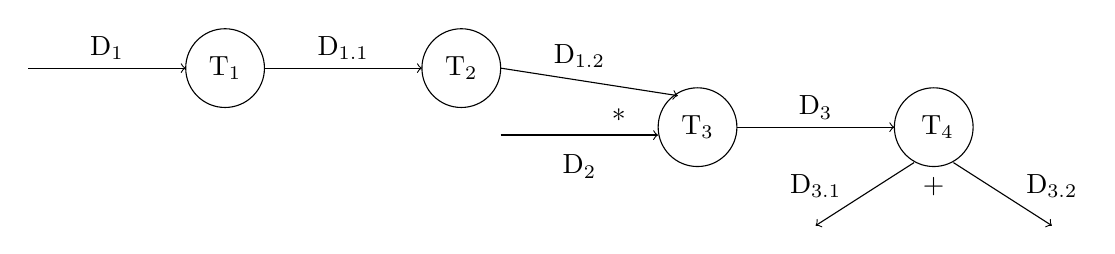
\begin{tikzpicture}
        \draw[->] (0,0) -- (2,0);
        \node at (1,0.25){D$_{1}$};
        \draw (2.5,0) circle (0.5);
        \node at (2.5,0) {T$_{1}$};
        
        \draw[->] (3,0) -- (5,0);
        \node at (4,0.25){D$_{1.1}$};
        \draw (5.5,0) circle (0.5);
        \node at (5.5,0) {T$_{2}$};

        \draw[->] (6,0) -- (8.25,-0.35);
        \node at (7,0.15){D$_{1.2}$};
        \draw (8.5,-0.75) circle (0.5);
        \node at (8.5,-0.75) {T$_{3}$};
        
        \draw[->] (6,-0.85) -- (8,-0.85);
        \draw[->] (9,-0.75) -- (11,-0.75);
        \node at (7.5,-0.65) {*};
        \node at (7,-1.25) {D$_{2}$};
        \node at (10,-0.5) {D$_{3}$};
        \draw (11.5,-0.75) circle (0.5);
        \node at (11.55,-0.75) {T$_{4}$};
        \draw[->] (11.25,-1.2) -- (10,-2);

        \node at (11.5,-1.5) {+};
        \draw[->] (11.75,-1.2) -- (13,-2);

        \node at (13,-1.5) {D$_{3.2}$};

        \node at (10,-1.5) {D$_{3.1}$};

    \end{tikzpicture}
\end{center}

\vspace{0.5cm}

\begin{prettyBox}{Note}{red}
    A DFD specifies the operations without detailing how they are performed. Each node in the diagram can be further described with another DFD, allowing for a hierarchical decomposition of processes.
\end{prettyBox}

\vspace{0.5cm}

\subsection*{\underline{Example :}}

\end{document}
